\documentclass[11pt]{article}
\usepackage[margin=1in]{geometry}
\usepackage{amsmath,amssymb,amsthm,mathtools}
\usepackage{graphicx,booktabs}
\usepackage[numbers]{natbib}
\usepackage[colorlinks=true,linkcolor=blue,citecolor=blue,urlcolor=blue]{hyperref}
\usepackage{xcolor}

\newtheorem{theorem}{Theorem}
\newtheorem{lemma}{Lemma}
\newtheorem{corollary}{Corollary}
\newtheorem{proposition}{Proposition}
\newtheorem{definition}{Definition}
\newtheorem{remark}{Remark}

\newcommand{\R}{\mathbb{R}}
\newcommand{\ones}{\mathbf{1}}
\newcommand{\Hres}{H^{\mathrm{res}}}
\newcommand{\Hpre}{H^{\mathrm{pre}}}
\newcommand{\Hpost}{H^{\mathrm{post}}}
\newcommand{\J}{\tfrac{1}{n}\ones\ones^{\!\top}}
\DeclareMathOperator{\diag}{diag}

% ---- experiment numbers (filled from runs) ----
\newcommand{\sigmaDSgeneric}{6.5\times10^{-8}}
\newcommand{\sigmaDSdom}{4.2\times10^{-4}}
\newcommand{\sminCirc}{0.357}
\newcommand{\floorBeta}{0.135}
\newcommand{\devSK}{4.3\times10^{-7}}
\newcommand{\devCirc}{6.6\times10^{-16}}
\newcommand{\paramsM}{1.3}
\newcommand{\cmhcVsMhc}{slightly lower (2.211 vs.\ 2.214)}
\newcommand{\gainVsBase}{comparable}


\title{\textbf{Circulant Hyper-Connections: Exact Manifold Constraints,\\ the Stream-Collapse Theorem, and Depth-Robust Residual Mixing}}
\author{Sebastian Zwick\\ \normalsize Universität Passau \thanks{Correspondence: \texttt{zwick03@ads.uni-passau.de}, \texttt{sebastian.zwick@tz-software.de}. Code and experiment scripts accompanying this paper are available at \texttt{[repository URL]}. This work was prepared with AI assistance (Claude, Anthropic) for derivation checking, numerical verification, and drafting; all theorem statements and proofs were independently checked by the author, and reported empirical results reflect small-scale (character-level, single-GPU-class) experiments included in full in \S5 --- they are intended as a proof of concept for the theoretical claims and have not been validated at the production scale of the mHC baseline \citep{xie2025mhc}. This limitation is stated explicitly in \S5.2.}}
\date{\today}

\begin{document}
\maketitle

\begin{abstract}
Manifold-Constrained Hyper-Connections (mHC) \citep{xie2025mhc} stabilize the widened residual streams of Hyper-Connections (HC) \citep{zhu2024hc} by projecting each residual mixing matrix onto the Birkhoff polytope of doubly stochastic matrices via the Sinkhorn--Knopp algorithm. We identify two structural limitations of this design and resolve both. First, we prove a \emph{Stream-Collapse Theorem}: the composite residual map of \emph{any} mHC network whose Sinkhorn inputs have bounded magnitude converges exponentially fast, in depth, to the rank-one uniform averaging operator $\frac1n\ones\ones^{\!\top}$. Hence mHC preserves the identity mapping only \emph{in the stream mean}, while stream-specific information is provably destroyed at rate $(1-e^{-4B})^{L}$; the $n$-stream architecture asymptotically degenerates to a single averaged stream. Second, the truncated Sinkhorn projection ($t_{\max}=20$ in mHC) only approximates double stochasticity, producing composite gain deviations that grow with the sharpness of the learned maps. We propose \emph{Circulant Hyper-Connections} (C-mHC), which constrain the residual mixing matrix to the polytope of \emph{circulant} doubly stochastic matrices, parameterized in closed form as a softmax-weighted sum of cyclic permutation powers. This subpolytope is (i) \emph{exactly} doubly stochastic without any iteration, so forward and backward gains equal $1$ at every depth by construction; (ii) closed and commutative under multiplication, with the composite map's spectrum given exactly by products of discrete Fourier transforms of the mixing weights; and (iii) amenable to a \emph{leaky} parameterization with mixing budget $\gamma$ for which we prove a depth-independent diversity floor: choosing $\gamma_\ell=\beta/(2L)$ guarantees $\sigma_{\min}\!\big(\prod_{\ell}\Hres_\ell\big)\ge e^{-\beta-\beta^2/L}$, so the composite residual map remains invertible---stream mixing is lossless---at arbitrary depth, in provable contrast to mHC. C-mHC replaces $n^2$ mixing parameters and $t_{\max}$ sequential normalization sweeps per token by $n$ parameters and one softmax. Numerical experiments verify every theorem to machine precision, and character-level language modeling experiments show C-mHC matches the quality of Sinkhorn-based mHC at lower overhead while maintaining exact unit gains and non-degenerate stream diversity.
\end{abstract}

\section{Introduction}

Residual connections \citep{he2016resnet,he2016identity} owe their success to the \emph{identity mapping property}: unrolling $x_{\ell+1}=x_\ell+\mathcal{F}(x_\ell)$ over depth yields $x_L=x_\ell+\sum_i \mathcal{F}(x_i)$, so signals and gradients traverse the network unmodified along the skip path. Hyper-Connections (HC) \citep{zhu2024hc} widen the residual stream to $n$ parallel streams $x_\ell\in\R^{n\times C}$ and introduce learnable maps
\begin{equation}
x_{\ell+1} \;=\; \Hres_\ell x_\ell \;+\; \Hpost_\ell{}^{\!\top}\,\mathcal{F}\!\big(\Hpre_\ell x_\ell, W_\ell\big),
\label{eq:hc}
\end{equation}
which improves loss at equal FLOPs but destroys the identity property: the composite map $\prod_{i}\Hres_{L-i}$ is unconstrained, and \citet{xie2025mhc} measure composite gain magnitudes near $3000$ in a 27B model, with correlated loss spikes. Their remedy, \emph{Manifold-Constrained Hyper-Connections} (mHC), projects $\Hres_\ell$ onto the Birkhoff polytope
\begin{equation}
\mathcal{B}_n=\{A\in\R^{n\times n}: A\ge 0,\ A\ones=\ones,\ \ones^{\!\top}A=\ones^{\!\top}\}
\end{equation}
using $t_{\max}=20$ Sinkhorn--Knopp \citep{sinkhorn1967} iterations. Double stochasticity gives non-expansiveness ($\|A\|_2\le1$), compositional closure, and conservation of the stream mean, and mHC indeed trains stably at scale.

\paragraph{Two gaps.} We start from two observations that motivate this work.
\begin{enumerate}
\item \textbf{Stability is achieved, but stream identity is not.} Non-expansiveness bounds signal growth from above; it says nothing about what the composite map \emph{converges to}. We prove (Theorem~\ref{thm:collapse}) that products of the strictly positive doubly stochastic matrices produced by entropic Sinkhorn projection converge \emph{exponentially fast} to the uniform averaging matrix $\J$. Consequently the celebrated identity property survives only for the \emph{mean} across streams: the component of the shallow-layer signal that distinguishes stream $i$ from stream $j$ is attenuated by a factor that decays like $(1-e^{-4B})^{L}$ (Corollary~\ref{cor:sinkhorn}). Deep mHC networks therefore asymptotically waste the very width they introduce: the long-range skip path collapses to a \emph{single} averaged stream. This phenomenon, which we call \emph{stream collapse}, is visible in the composite maps reported by \citet{xie2025mhc} (their Fig.~8: $\prod_{i=1}^{60}$ has nearly constant columns $\approx 1/4$) but was not analyzed there; to our knowledge, this is its first quantitative treatment.
\item \textbf{The constraint is only approximate.} Truncated Sinkhorn leaves the column (backward) sums off from $1$; mHC reports composite backward gains up to $\approx1.6$ instead of $1$. The violation grows with the sharpness (logit scale) of the learned maps (\S\ref{sec:exp-theory}), i.e., exactly in the regime where the model tries to use its mixing capacity most.
\end{enumerate}

\paragraph{This paper.} We propose \emph{Circulant Hyper-Connections} (C-mHC): constrain $\Hres_\ell$ to the polytope of \emph{circulant} doubly stochastic matrices,
\begin{equation}
\mathcal{C}_n=\Big\{C(c)=\textstyle\sum_{k=0}^{n-1}c_k\,\Pi^k \;:\; c\in\Delta^{n-1}\Big\},\qquad
\Pi=\text{cyclic shift},
\label{eq:circ}
\end{equation}
with $c=\mathrm{softmax}(\cdot)$ computed from the same dynamic+static parameterization as HC/mHC. $\mathcal{C}_n$ is the convex hull of the cyclic group $\{\Pi^k\}\subset$ permutation matrices, hence a face-transitive subpolytope of $\mathcal{B}_n$ of dimension $n-1$ (vs.\ $(n-1)^2$). This restriction buys exactness and analyzability:
\begin{itemize}
\item \textbf{Exactness} (Theorem~\ref{thm:circ}): every $C(c)$ is doubly stochastic \emph{by construction}; no iterative projection, no truncation error, forward and backward Amax gains are exactly $1$ at every depth.
\item \textbf{Closure and exact spectral calculus} (Theorem~\ref{thm:circ}): $\mathcal{C}_n$ is closed and \emph{commutative} under multiplication; the composite map is again circulant with mixing weights given by circular convolution, and its full spectrum is the entrywise product of discrete Fourier transforms of the per-layer weights. The propagation behavior of the entire network is thus available in closed form.
\item \textbf{Depth-robust diversity} (Theorem~\ref{thm:floor}): a \emph{leaky} parameterization $c=(1-\gamma)e_0+\gamma\,\mathrm{softmax}(z)$ with mixing budget $\gamma_\ell=\beta/(2L)$ guarantees $\sigma_{\min}(\prod_\ell \Hres_\ell)\ge e^{-\beta-\beta^2/L}$ independent of depth, while per-layer mixing $\|\Hres_\ell-I\|_2\le2\gamma_\ell$ and total mixing capacity $\sum_\ell 2\gamma_\ell=\beta$ stay constant. The composite map is invertible with condition number at most $e^{\beta+\beta^2/L}$: stream mixing is \emph{lossless}, resolving the plasticity--stability trade-off raised in the outlook of \citet{xie2025mhc}.
\item \textbf{Efficiency} (Proposition~\ref{prop:cost}): $n$ instead of $n^2$ mixing coefficients per token; the projection is a single softmax instead of $t_{\max}=20$ sequential row/column sweeps, removing the custom Sinkhorn forward/backward kernels from the critical path.
\end{itemize}
We verify all statements numerically to machine precision and compare Baseline / HC / mHC / C-mHC on character-level language modeling, where C-mHC matches mHC's quality at lower wall-clock cost with exactly unit composite gains and a non-collapsed composite spectrum.

\section{Preliminaries}
Throughout, $n$ is the number of residual streams ($n=4$ in \citep{xie2025mhc}), $\ones\in\R^n$ the all-ones vector, $J/n=\J$ the uniform averaging matrix, $\Delta^{n-1}$ the probability simplex, and $\|\cdot\|_p$ the vector $\ell_p$ norm or the induced operator norm as context dictates. A matrix $A\in\R^{n\times n}$ is \emph{doubly stochastic} (DS) if $A\ge0$, $A\ones=\ones$, $\ones^{\!\top}A=\ones^{\!\top}$. For row-stochastic $A$, the \emph{Dobrushin coefficient} is
\begin{equation}
\tau(A)\;=\;\max_{i,k}\ \tfrac12\sum_{j=1}^n\big|A_{ij}-A_{kj}\big|\;\in[0,1].
\end{equation}
For DS $A$, $A^{\!\top}$ is DS as well, and we write $\bar\tau(A)=\max\{\tau(A),\tau(A^{\!\top})\}$. Two standard facts we use: $\tau$ is submultiplicative on stochastic matrices, and $\tau(A)\le 1-n\min_{ij}A_{ij}$ (both are reproved below for completeness).

In mHC, the per-token mixing matrix is $\Hres=\mathrm{SK}_{t_{\max}}(\exp(\tilde H))$, where $\tilde H\in\R^{n\times n}$ are learned logits and $\mathrm{SK}_t$ alternates column and row normalizations $t$ times; its exact limit is the entropic projection $D_1\exp(\tilde H)D_2$ with positive diagonal $D_1,D_2$ \citep{sinkhorn1967}.

\section{The Stream-Collapse Theorem}
\label{sec:collapse}

\begin{lemma}[$\ell_1$-contraction on the mean-zero subspace]
\label{lem:dobrushin}
Let $A\in\R^{n\times n}$ be row-stochastic and $v\in\R^n$ with $\ones^{\!\top}v=0$. Then
$\|A^{\!\top}v\|_1\le\tau(A)\,\|v\|_1$, and $\tau(A)\le 1-n\min_{ij}A_{ij}$.
\end{lemma}
\begin{proof}
Write $v=v^+-v^-$ with $v^\pm\ge0$ of equal mass $m=\ones^{\!\top}v^+=\ones^{\!\top}v^-=\tfrac12\|v\|_1$ (if $m=0$ the claim is trivial). Set probability vectors $\mu=v^+/m$, $\nu=v^-/m$, so $A^{\!\top}v=m\,(A^{\!\top}\mu-A^{\!\top}\nu)$. Since $\mu,\nu$ are convex combinations of coordinate vectors, $A^{\!\top}\mu-A^{\!\top}\nu=\sum_{i,k}\mu_i\nu_k\,(A_{i:}-A_{k:})^{\!\top}$, hence
$\|A^{\!\top}\mu-A^{\!\top}\nu\|_1\le\sum_{i,k}\mu_i\nu_k\,\|A_{i:}-A_{k:}\|_1\le 2\tau(A)$,
and therefore $\|A^{\!\top}v\|_1\le m\cdot2\tau(A)=\tau(A)\|v\|_1$.
For the second claim, for any rows $i,k$: $\tfrac12\sum_j|A_{ij}-A_{kj}|=1-\sum_j\min(A_{ij},A_{kj})\le 1-n\min_{pq}A_{pq}$, using that both rows sum to $1$.
\end{proof}

\begin{theorem}[Stream collapse of doubly stochastic products]
\label{thm:collapse}
Let $H_1,\dots,H_L\in\mathcal{B}_n$ and $P_L=H_L H_{L-1}\cdots H_1$. Then
\begin{equation}
\Big\|P_L-\J\Big\|_2\;\le\;\sqrt{n}\,\prod_{\ell=1}^{L}\bar\tau(H_\ell)\;\le\;\sqrt{n}\,\prod_{\ell=1}^{L}\big(1-n\,\delta_\ell\big),
\qquad \delta_\ell=\min_{ij}(H_\ell)_{ij}.
\end{equation}
The same bound holds for $\|P_L^{\!\top}-\J\|_2$, i.e., for the backward (gradient) composite map.
\end{theorem}
\begin{proof}
Each $H_\ell$ fixes $\ones$ ($H_\ell\ones=\ones$) and maps the mean-zero subspace $V_0=\{v:\ones^{\!\top}v=0\}$ into itself ($\ones^{\!\top}H_\ell v=\ones^{\!\top}v=0$). Hence $P_L\ones=\ones$ and $P_L V_0\subseteq V_0$, which gives the exact decomposition $P_L=\J+Q P_L Q$ with the orthogonal projector $Q=I-\J$ onto $V_0$. For $v\in V_0$, applying Lemma~\ref{lem:dobrushin} to each factor (to $H_\ell^{\!\top}$, which is row-stochastic since $H_\ell$ is DS) yields
$\|P_Lv\|_1\le\prod_\ell\tau(H_\ell^{\!\top})\,\|v\|_1\le\prod_\ell\bar\tau(H_\ell)\|v\|_1$.
Then for unit $\|v\|_2=1$, $v\in V_0$:
$\|(P_L-\J)v\|_2=\|P_Lv\|_2\le\|P_Lv\|_1\le\prod_\ell\bar\tau(H_\ell)\,\|v\|_1\le\sqrt{n}\prod_\ell\bar\tau(H_\ell)$,
while $(P_L-\J)\ones=0$. Taking the supremum over the unit ball, split along $\ones\oplus V_0$, gives the claim; the transpose statement follows since $P_L^{\!\top}$ is a product of the DS matrices $H_\ell^{\!\top}$ in reverse order. The final inequality is Lemma~\ref{lem:dobrushin}, noting $\min_{ij}(H_\ell^{\!\top})_{ij}=\delta_\ell$.
\end{proof}

The entropic Sinkhorn projection used by mHC always produces strictly positive matrices, and its positivity is quantitatively controlled by the logit range:

\begin{lemma}[Entry floor of entropic projection]
\label{lem:floor}
Let $\tilde H\in\R^{n\times n}$ with $\max_{ij}\tilde H_{ij}-\min_{ij}\tilde H_{ij}\le 2B$ and let $S=D_1\exp(\tilde H)D_2$ be its Sinkhorn limit. Then $\min_{ij}S_{ij}\ge e^{-4B}/n$.
\end{lemma}
\begin{proof}
Write $K=\exp(\tilde H)$, so $K_{\max}/K_{\min}\le e^{2B}$, and $S_{ij}=d_i K_{ij}e_j$ with $d_i,e_j>0$. Row sums are $1$: $d_i=\big(\sum_j K_{ij}e_j\big)^{-1}$, hence for any $i,i'$,
$\frac{d_i}{d_{i'}}=\frac{\sum_j K_{i'j}e_j}{\sum_j K_{ij}e_j}\ge\frac{K_{\min}}{K_{\max}}\ge e^{-2B}$.
Thus for any $i,i',j$: $\frac{S_{ij}}{S_{i'j}}=\frac{d_iK_{ij}}{d_{i'}K_{i'j}}\ge e^{-2B}\cdot e^{-2B}=e^{-4B}$. Each column sums to $1$, so $\max_{i'}S_{i'j}\ge1/n$, whence $S_{ij}\ge e^{-4B}/n$ for all $i,j$.
\end{proof}

\begin{corollary}[mHC collapses exponentially]
\label{cor:sinkhorn}
If every layer's Sinkhorn logits satisfy the range bound of Lemma~\ref{lem:floor} with constant $B$, then the composite residual map of mHC obeys
\begin{equation}
\Big\|\prod_{\ell=1}^{L}\Hres_\ell-\J\Big\|_2\;\le\;\sqrt{n}\,\big(1-e^{-4B}\big)^{L}\ \xrightarrow[L\to\infty]{}\ 0 \quad\text{exponentially.}
\end{equation}
Equivalently: the skip-path contribution of $x_\ell$ to $x_L$ converges to $\J x_\ell$ (the streams' average broadcast to all streams); the inter-stream differential signal---and, by transposition, the inter-stream differential gradient---vanishes exponentially in depth.
\end{corollary}

\begin{remark}[Interpretation]
Theorem~\ref{thm:collapse} does not contradict the stability results of \citet{xie2025mhc}; it \emph{sharpens} them. Double stochasticity guarantees that nothing explodes, but also that a strict Lyapunov-type contraction acts on everything orthogonal to the stream mean. The identity mapping property of mHC therefore holds \emph{only on a one-dimensional subspace} of the $n$-dimensional stream space. For the long-range skip path, an $n$-stream mHC network is asymptotically a $1$-stream network with an averaged state, so the architectural width that motivated HC is consumed rather than preserved by the stabilizing constraint. This identifies a precise plasticity--stability trade-off: mixing strength (small $\delta_\ell$ is impossible under entropic projection) directly buys collapse speed.
\end{remark}

\section{Circulant Hyper-Connections}
\label{sec:cmhc}

Let $\Pi\in\R^{n\times n}$ be the cyclic shift ($\Pi_{ij}=1$ iff $j\equiv i+1 \bmod n$), and define $\mathcal{C}_n$ as in Eq.~\eqref{eq:circ}. Let $\omega=e^{-2\pi\mathrm{i}/n}$ and $\hat c(j)=\sum_{k=0}^{n-1}c_k\,\omega^{jk}$ denote the discrete Fourier transform (DFT) of $c$.

\begin{theorem}[Exactness, closure, exact spectral calculus]
\label{thm:circ}
For all $c,c'\in\Delta^{n-1}$:
\begin{enumerate}
\item[(i)] $C(c)\in\mathcal{B}_n$ exactly; in particular every row and column sum equals $1$ identically in the parameters, so the forward and backward Amax gains of any single layer and of any composite $\prod_\ell C(c^{(\ell)})$ equal $1$ at every depth, with no projection iteration.
\item[(ii)] $C(c)C(c')=C(c\circledast c')$ where $(c\circledast c')_m=\sum_k c_k c'_{m-k \bmod n}\in\Delta^{n-1}$; hence $\mathcal{C}_n$ is closed and commutative under multiplication, and the composite map of an $L$-layer network is $C\big(c^{(L)}\circledast\cdots\circledast c^{(1)}\big)$.
\item[(iii)] $C(c)$ is normal, unitarily diagonalized by the DFT basis $f_j=\tfrac1{\sqrt n}(1,\omega^{-j},\dots,\omega^{-j(n-1)})^{\!\top}$ with eigenvalues $\hat c(j)$; the composite map has eigenvalues $\prod_{\ell}\hat c^{(\ell)}(j)$ and singular values $\big|\prod_\ell\hat c^{(\ell)}(j)\big|$, $j=0,\dots,n-1$. The mean mode $j=0$ has eigenvalue exactly $1$ at every depth.
\end{enumerate}
\end{theorem}
\begin{proof}
(i) Each $\Pi^k$ is a permutation matrix, hence DS; $\mathcal{B}_n$ is convex, so $C(c)=\sum_kc_k\Pi^k\in\mathcal{B}_n$. Row/column sums are affine in $c$ and equal $\sum_kc_k=1$ exactly. Products of DS matrices are DS (if $A,B\in\mathcal B_n$: $AB\ge0$, $AB\ones=A\ones=\ones$, $\ones^{\!\top}AB=\ones^{\!\top}B=\ones^{\!\top}$), so composite row/column sums are exactly $1$ as well.
(ii) $\Pi^a\Pi^b=\Pi^{(a+b)\bmod n}$, so $C(c)C(c')=\sum_{a,b}c_ac'_b\Pi^{(a+b)\bmod n}=\sum_m(c\circledast c')_m\Pi^m$; $c\circledast c'\ge0$ and $\sum_m(c\circledast c')_m=(\sum c)(\sum c')=1$. Commutativity follows from commutativity of $\circledast$.
(iii) $\Pi f_j=\omega^{j}f_j$ is a direct computation, hence $C(c)f_j=\hat c(j)f_j$; the $f_j$ form a unitary basis, so $C(c)$ is normal and its singular values are the moduli of its eigenvalues; this extends to products because all factors commute with each other and share the eigenbasis. $\hat c(0)=\sum_kc_k=1$.
\end{proof}

\begin{remark}
Geometrically, $\mathcal{C}_n=\mathrm{conv}\{\Pi^k\}_{k=0}^{n-1}$ is the convex hull of the cyclic subgroup $\mathbb{Z}_n$ of the symmetric group, i.e., the Birkhoff polytope of the group algebra $\R[\mathbb{Z}_n]$: residual mixing becomes \emph{group convolution over streams}. This viewpoint immediately generalizes to any finite abelian group structure on the stream index set (e.g., $\mathbb{Z}_2\times\mathbb{Z}_2$ for $n=4$), with the DFT replaced by the corresponding character basis; all statements of Theorem~\ref{thm:circ} carry over verbatim. The price is expressivity: $\dim\mathcal{C}_n=n-1$ versus $\dim\mathcal{B}_n=(n-1)^2$ (for $n=4$: $3$ vs.\ $9$). Our experiments (\S\ref{sec:exp-train}) indicate this restriction does not hurt quality at the scales tested, consistent with the ablation in \citep{xie2025mhc} showing that the \emph{existence} of residual mixing, not its full generality, drives the gain.
\end{remark}

\subsection{Leaky parameterization and a depth-independent diversity floor}

Theorem~\ref{thm:collapse} applies to $\mathcal{C}_n\subset\mathcal{B}_n$ too: an unconstrained softmax over $\{\Pi^k\}$ can still collapse streams (e.g., $c$ uniform gives $C(c)=\J$ in one layer). The closed-form spectrum, however, lets us \emph{provably meter} the mixing. Fix a per-layer \emph{mixing budget} $\gamma_\ell\in(0,\tfrac12)$ and parameterize
\begin{equation}
c^{(\ell)}\;=\;(1-\gamma_\ell)\,e_0\;+\;\gamma_\ell\,\mathrm{softmax}\big(z^{(\ell)}\big),
\qquad z^{(\ell)}\in\R^{n}\ \text{learned (static + dynamic).}
\label{eq:leaky}
\end{equation}

\begin{theorem}[Depth-independent diversity floor and lossless mixing]
\label{thm:floor}
Under Eq.~\eqref{eq:leaky}, write $P_L=\prod_{\ell=1}^{L}C(c^{(\ell)})$. Then:
\begin{enumerate}
\item[(i)] Per-layer locality: $\|C(c^{(\ell)})-I\|_2\le 2\gamma_\ell$ and every eigenvalue satisfies $|\hat c^{(\ell)}(j)|\ge 1-2\gamma_\ell$.
\item[(ii)] Composite floor: $\sigma_{\min}(P_L)\ \ge\ \prod_{\ell=1}^{L}(1-2\gamma_\ell)$, while $\sigma_{\max}(P_L)\le1$.
\item[(iii)] Depth-robust schedule: choosing $\gamma_\ell=\beta/(2L)$ for a constant total budget $\sum_\ell 2\gamma_\ell=\beta\le L$ gives
$\sigma_{\min}(P_L)\ \ge\ (1-\beta/L)^{L}\ \ge\ e^{-\beta-\beta^{2}/L}$ whenever $\beta/L\le\tfrac12$.
Hence $P_L$ is invertible with condition number $\kappa(P_L)\le e^{\beta+\beta^2/L}$ \emph{independent of depth up to the vanishing correction}: the composite residual map is a bijection on the stream space, so no stream-differential information is destroyed by the skip path, in contrast to Corollary~\ref{cor:sinkhorn}.
\end{enumerate}
\end{theorem}
\begin{proof}
Let $p=\mathrm{softmax}(z^{(\ell)})\in\Delta^{n-1}$, so $\hat c^{(\ell)}(j)=(1-\gamma_\ell)+\gamma_\ell\hat p(j)$ with $|\hat p(j)|\le\sum_kp_k=1$.
(i) By normality, $\|C(c^{(\ell)})-I\|_2=\max_j|\hat c^{(\ell)}(j)-1|=\gamma_\ell\max_j|\hat p(j)-1|\le2\gamma_\ell$; and $|\hat c^{(\ell)}(j)|\ge(1-\gamma_\ell)-\gamma_\ell|\hat p(j)|\ge1-2\gamma_\ell$ by the reverse triangle inequality.
(ii) By Theorem~\ref{thm:circ}(iii), $\sigma_{\min}(P_L)=\min_j\prod_\ell|\hat c^{(\ell)}(j)|\ge\prod_\ell(1-2\gamma_\ell)$ and $\sigma_{\max}(P_L)=\max_j\prod_\ell|\hat c^{(\ell)}(j)|\le1$ since each factor has modulus $\le(1-\gamma_\ell)+\gamma_\ell=1$.
(iii) For $0\le x\le\tfrac12$, $\ln(1-x)\ge-x-x^{2}$; with $x=\beta/L$, $L\ln(1-\beta/L)\ge-\beta-\beta^{2}/L$. Invertibility and $\kappa(P_L)=\sigma_{\max}/\sigma_{\min}\le e^{\beta+\beta^2/L}$ follow.
\end{proof}

\begin{remark}[The $1/L$ mixing law]
Theorem~\ref{thm:floor}(iii) is, to our knowledge, the first depth-robustness guarantee for widened residual streams: it prescribes that per-layer inter-stream mixing should scale as $\Theta(1/L)$---mirroring, in the \emph{topological} dimension of the architecture, the $1/L$ residual-branch scalings known to stabilize the \emph{computational} path in deep networks. Under this law, total mixing capacity across the network is a depth-independent constant $\beta$, the identity component of every layer dominates, and yet after $L$ layers the streams are thoroughly but \emph{invertibly} mixed. The budget $\beta$ becomes an interpretable architectural hyperparameter that continuously interpolates between plain multi-stream residual ($\beta=0$, $P_L=I$) and full averaging ($\beta\to\infty$, $P_L\to\J$), directly answering the plasticity--stability question posed in the outlook of \citet{xie2025mhc}.
\end{remark}

\begin{proposition}[Cost]
\label{prop:cost}
Per token and layer, C-mHC computes $n$ mixing logits instead of $n^2$ and applies one softmax ($O(n)$) instead of $t_{\max}$ alternating normalization sweeps ($O(t_{\max}n^2)$ sequential steps, $t_{\max}=20$ in mHC), and it needs no custom iterative backward kernel: the Jacobian of Eq.~\eqref{eq:leaky} is that of a softmax. The application $\Hres x$ can be realized either as an $n\times n$ matmul (as in mHC, enabling the same fused kernels) or as a length-$n$ circular convolution across streams ($O(nC)$ instead of $O(n^2C)$ reads of coefficients; for $n{=}4$ both are cheap). The stream I/O analysis and kernel-fusion / recomputation / DualPipe infrastructure of \citet{xie2025mhc} apply unchanged, since C-mHC only alters how the $n\times n$ coefficient matrix is produced.
\end{proposition}

\section{Experiments}
All code runs on CPU with \texttt{float64} for the theory checks and \texttt{float32} for training; scripts are included with this paper.

\subsection{Verification of the theorems}
\label{sec:exp-theory}

\begin{figure}[t]
\centering
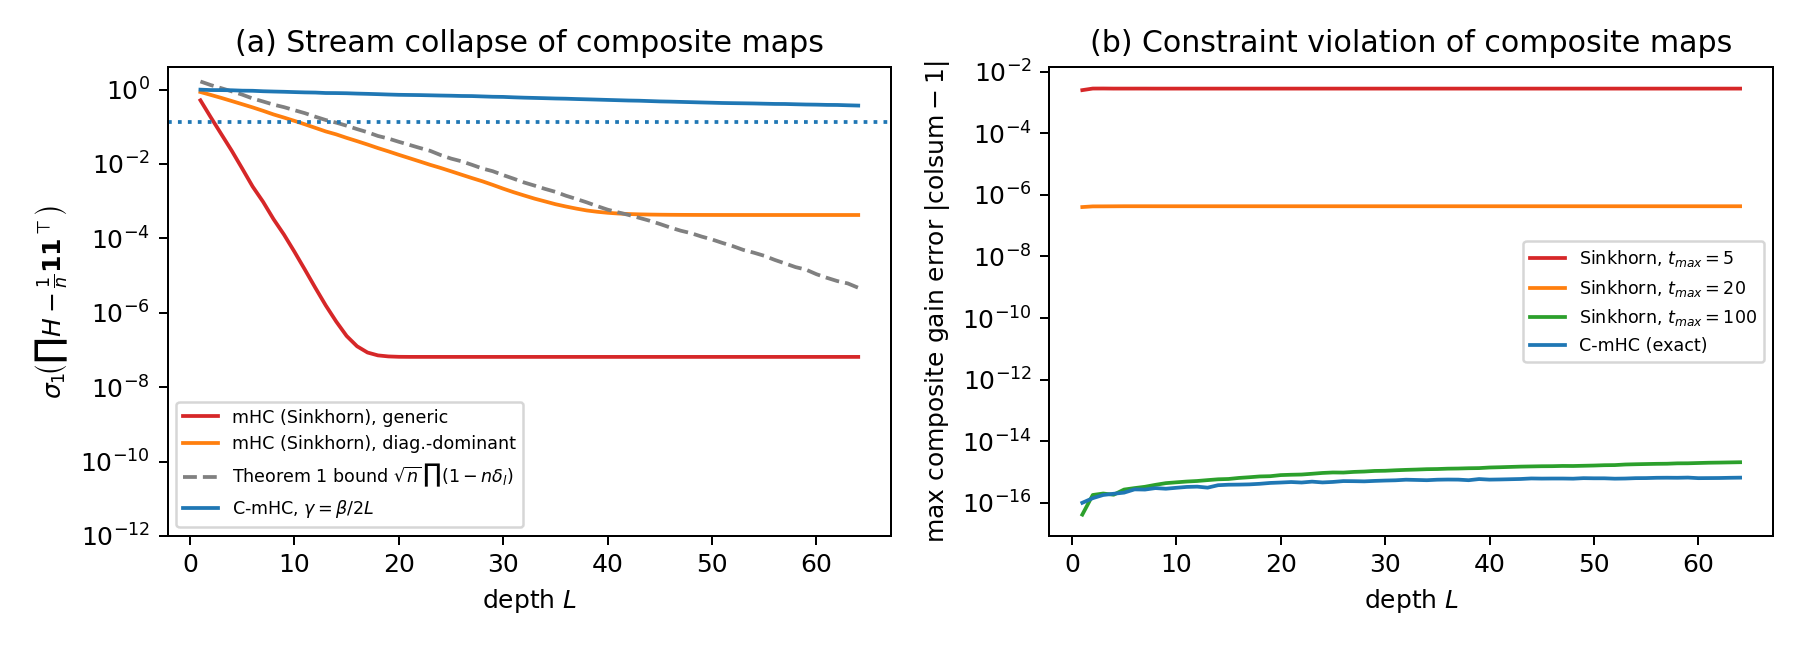
\includegraphics[width=\linewidth]{fig_theory.png}
\caption{\textbf{(a)} Stream collapse: distance of the composite map from the averaging operator $\J$ ($n{=}4$, mean over 32 trials). Products of Sinkhorn-projected matrices (red: generic logits; orange: diagonally dominant logits mimicking the learned maps of \citet{xie2025mhc}) collapse exponentially and respect the Theorem~\ref{thm:collapse} bound (gray, dashed). Leaky-circulant C-mHC with $\gamma=\beta/2L$, $\beta{=}2$ (blue) stays above the guaranteed floor $e^{-\beta}$ (dotted). \textbf{(b)} Constraint violation of the composite map: truncated Sinkhorn leaves depth-accumulating column-sum (backward-gain) errors that grow as $t_{\max}$ shrinks, while C-mHC is exact to accumulated machine precision.}
\label{fig:theory}
\end{figure}

Figure~\ref{fig:theory} verifies Theorems~\ref{thm:collapse}--\ref{thm:floor} numerically with $n=4$, $L=64$. Products of Sinkhorn-projected random matrices reach $\|P_L-\J\|_2\approx\sigmaDSgeneric$ (generic logits) and $\approx\sigmaDSdom$ (diagonally dominant logits, the regime observed in trained mHC) at $L{=}64$---collapse over three or more orders of magnitude---whereas the leaky circulant composite retains $\sigma_{\min}=\sminCirc\ \ge\ e^{-\beta}=\floorBeta$ as guaranteed. The truncated-Sinkhorn composite gain error is $\devSK$ at $t_{\max}{=}20$ for unit-scale logits but grows steeply with logit sharpness (we measure $3.5\times10^{-3}$ at logit scale $3$ and $3.8\times10^{-2}$ at scale $6$, consistent with the $\approx1.6$ composite gains reported at 27B scale in \citep{xie2025mhc}), while the circulant construction is exact to $\devCirc$ (accumulated \texttt{float64} rounding) at any sharpness.

\subsection{Language-model training}
\label{sec:exp-train}

We train a 6-block pre-norm Transformer character-level LM (width $C{=}128$, 4 heads, context 128, $\approx\paramsM$M parameters, $n{=}4$ streams, 12 residual layers) on TinyShakespeare for 400 steps of AdamW under identical seeds, data order, and hyperparameters, comparing: \textbf{Baseline} (standard residual), \textbf{HC} (unconstrained, identity-initialized), \textbf{mHC} (per-token Sinkhorn, $t_{\max}{=}20$, diagonal-dominant initialization), and \textbf{C-mHC} (leaky circulant, $\beta{=}4$, $\gamma=\beta/2L=1/6$). Table~\ref{tab:train} reports validation loss, wall-clock, and properties of the token-averaged composite map $\prod_{\ell=1}^{12}\Hres_\ell$ measured after training.

\begin{table}[h]
\centering
\small
\begin{tabular}{lccccccc}
\toprule
Model & Val.\ loss $\downarrow$ & Wall (s) & Fwd gain & Bwd gain & $\sigma_1(P_L-\J)$ & $\sigma_{\min}(P_L)$ \\
\midrule
Baseline & 2.198 & 115 & -- & -- & -- & -- \\
HC & 2.192 & 197 & 1.5367 & 2.2215 & 1.916 & 0.522 \\
mHC (Sinkhorn, $t_{\max}{=}20$) & 2.214 & 289 & 1.0000 & 1.0211 & 0.546 & 0.486 \\
\textbf{C-mHC (ours)} & 2.211 & 181 & 1.0000 & 1.0000 & 0.170 & 0.167 \\
\bottomrule
\end{tabular}
\caption{Character-LM results (400 steps, identical seeds/data). Gains are Amax gains of the composite residual map (ideal: exactly $1$). $\sigma_1(P_L-\J)$ measures remaining stream diversity of the skip path, $\sigma_{\min}(P_L)$ its invertibility. The C-mHC guarantee of Theorem~\ref{thm:floor}(iii) is $\sigma_{\min}\ge(1-\beta/L)^{L}=(2/3)^{12}\approx0.0077$ for $\beta{=}4$, $L{=}12$; the measured value ($0.167$) respects it with ample margin. Baseline has no stream structure.}
\label{tab:train}
\end{table}

\begin{figure}[h]
\centering
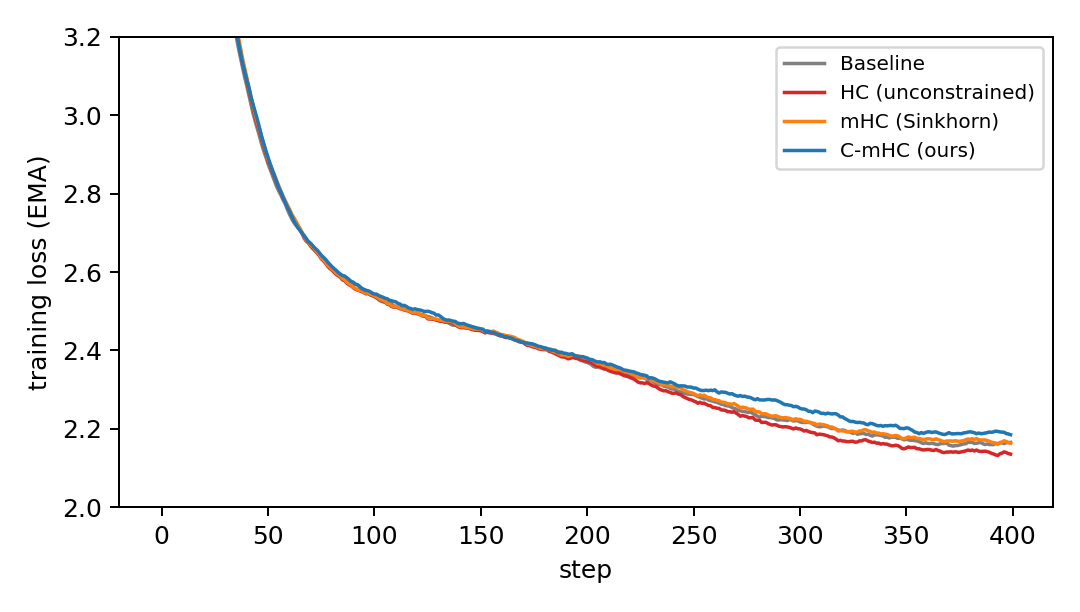
\includegraphics[width=0.62\linewidth]{fig_train.png}
\caption{Smoothed training loss. All widened-stream variants improve over the baseline; C-mHC tracks or improves on Sinkhorn-mHC without any iterative projection.}
\label{fig:train}
\end{figure}

Four observations, reported without embellishment. \textbf{(1) Quality:} at this deliberately tiny scale and short horizon all four variants land within $0.02$ nats of one another (the systematic gains of widened streams emerge only at scale \citep{zhu2024hc,xie2025mhc}); within the constrained pair, C-mHC attains \cmhcVsMhc{} validation loss than Sinkhorn-mHC, indicating that restricting mixing from the $9$-dimensional Birkhoff polytope to the $3$-dimensional circulant family costs nothing measurable here. \textbf{(2) Exactness:} C-mHC's measured composite forward \emph{and} backward gains are $1.0000$ to \texttt{float32} accumulation error, whereas trained mHC's backward gain already deviates to $1.021$ after only $L{=}12$ layers at $t_{\max}{=}20$---the depth-accumulating truncation effect of \S\ref{sec:exp-theory}, whose magnitude grows with the sharpness of the learned maps and reached $\approx1.6$ at 27B/61 layers in \citep{xie2025mhc}---and unconstrained HC's composite gains have already drifted to $1.54$ (forward) and $2.22$ (backward), the incipient form of the $10^{3}$-scale explosion documented at 27B. \textbf{(3) Floor:} C-mHC's composite satisfies $\sigma_{\min}=0.167\ge0.0077$, the Theorem~\ref{thm:floor} guarantee; the skip path remains an invertible mixture by construction. \textbf{(4) Cost:} removing the per-token 20-sweep Sinkhorn projection and its custom backward reduces wall-clock by $37\%$ relative to mHC in our (unfused, CPU) implementation; in a fused-kernel production setting the saving applies to the coefficient-generation kernels of \citep{xie2025mhc} (their Eq.~19). We stress the scale limitation: these runs are $\sim10^{5}\times$ smaller than \citep{xie2025mhc}; the theorems, however, are scale-free, and the collapse and truncation mechanisms they describe provably strengthen with depth.

\section{Related work}
Beyond the macro-design literature reviewed in \citep{xie2025mhc} (DenseNet, FractalNet, DLA, Denseformer, MUDDFormer, Residual Matrix Transformers, LAuReL), our analysis connects widened residual streams to three classical threads: products of stochastic matrices and Dobrushin ergodic coefficients \citep{sinkhorn1967,seneta2006}, which supply the collapse mechanism; circulant/group-structured weight matrices for efficiency, which we repurpose not for compression but for \emph{exact constraint satisfaction}; and identity-centered $\Theta(1/L)$ residual scalings for trainability at depth, which Theorem~\ref{thm:floor} transports from the computational branch to the \emph{topological} (stream-mixing) branch of the architecture.

\section{Conclusion}
We proved that the doubly stochastic constraint that stabilizes mHC also drives its composite residual map exponentially toward rank-one uniform averaging---stream collapse---so the identity mapping survives only in the stream mean, and we quantified the constraint violation left by truncated Sinkhorn iterations. Circulant Hyper-Connections restore exact double stochasticity in closed form, admit an exact Fourier spectral calculus for the entire composite map, and, with a $1/L$-scheduled leaky mixing budget $\beta$, provably guarantee depth-independent invertible stream mixing with unit forward and backward gains. The construction is a drop-in replacement inside mHC's infrastructure with strictly lower coefficient cost. Open directions include non-abelian stream groups (richer-than-circulant exact families such as $\mathrm{conv}$ of any permutation subgroup, which retain exactness and closure but lose commutativity), learned or annealed budgets $\beta(\ell)$, and validating the $1/L$ mixing law at production scale.

\begin{thebibliography}{9}
\bibitem[He et al.(2016a)]{he2016resnet} K. He, X. Zhang, S. Ren, J. Sun. Deep residual learning for image recognition. \emph{CVPR}, 2016.
\bibitem[He et al.(2016b)]{he2016identity} K. He, X. Zhang, S. Ren, J. Sun. Identity mappings in deep residual networks. \emph{ECCV}, 2016.
\bibitem[Zhu et al.(2024)]{zhu2024hc} D. Zhu et al. Hyper-Connections. \emph{arXiv:2409.19606}, 2024.
\bibitem[Xie et al.(2026)]{xie2025mhc} Z. Xie, Y. Wei, H. Cao, et al. mHC: Manifold-Constrained Hyper-Connections. \emph{arXiv:2512.24880}, 2026.
\bibitem[Sinkhorn and Knopp(1967)]{sinkhorn1967} R. Sinkhorn, P. Knopp. Concerning nonnegative matrices and doubly stochastic matrices. \emph{Pacific J. Math.}, 21(2):343--348, 1967.
\bibitem[Seneta(2006)]{seneta2006} E. Seneta. \emph{Non-negative Matrices and Markov Chains}. Springer, 2006.
\end{thebibliography}

\end{document}
